\documentclass{article}
\usepackage{amsmath}
\usepackage{amssymb}
\usepackage{graphicx}
\usepackage{hyperref}
\usepackage[version=4]{mhchem}


\begin{document}
\section*{Problem}
As shown in the figure, \(B D, C E\) are the altitudes on \(A C, A B\) of \(\triangle A B C\), respectively. \(E M \perp B D\) at \(M, D N \perp C E\) at \(N\). Show that \(M N / / B C\).\\
\centering
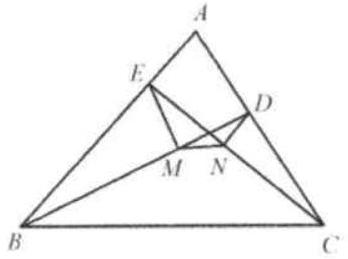
\includegraphics[width=\textwidth]{images/207(3).jpg}

\section*{Solution}
\(\angle B E C=\angle B D C=90^{\circ}\).\\
Thus points \(B, C, D\), and \(E\) are concyclic.\\
Draw the circle as shown.\\
So \(\angle C E D=\angle C B D=\alpha\) (they face the same arc \(C D\) ).\\
\(\angle E M D=\angle E N D=90^{\circ}\).\\
Thus points \(E, M, N\), and \(D\) are concyclic.\\
So \(\angle N E D=\angle N M D=\alpha\) (they face the same chord \(D N\) ).\\
Since \(\angle C B D=\angle N M D=\alpha, M N / / B C\).\\
\centering
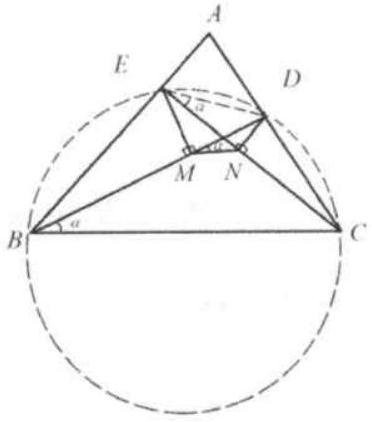
\includegraphics[width=\textwidth]{images/210(2).jpg}

\end{document}
